%Capitulo 4 - análise e resultados%

\thispagestyle{fancy}

\section{Implementação do sistema}
\label{impl_sist}

Para a realização dos experimentos práticos apenas ferramentas livres foram utilizadas, em que um codec (codificador/decodificador) H.261 simplificado e o método de quantização perceptual inter-adaptativa (seção \ref{QIBSVH}) foram implementados em Python \cite{pythonbrasil} com auxílio da biblioteca OpenCV \cite{opencv}.

\section{Conjunto de teste}
\label{Conj_teste}

A análise do método de quantização perceptual \cite{Li_humanvisual} utilizado neste trabalho consiste em compará-lo com o utilizado no codificador H.261 padrão com diferentes condições. Para este procedimento, quatro vídeos  com diferentes características, obtidos em \cite{xiph_org}, serão utilizados (Tabela \ref{descr_videos}), de forma a analisar a compressão e a qualidade visual alcançada.

\begin{table}[!ht]
\centering
\begin{tabular}{|c|c|c|c|c|}
\hline
Vídeos       & \begin{tabular}[c]{@{}c@{}}Atividade\\ Temporal\end{tabular} & \begin{tabular}[c]{@{}c@{}}Duração\\ (seg) \end{tabular} & Resolução & FPS \\ \hline
Akiyo\_cif   & Baixa                                                        & 12            & 352 x 288 & 25  \\ \hline
Ice\_cif     & Baixa & 8             & 352 x 288 & 30  \\ \hline
Stefan\_cif  & Média & 3             & 352 x 288 & 25  \\ \hline
Foreman\_cif & Alta                                                         & 12            & 352 x 288 & 25  \\ \hline
\end{tabular}
\caption{Descrição dos vídeos.}
\label{descr_videos}
\end{table}

\section{Procedimento experimental}
\label{proc_experimental}

Os experimentos realizados tem dois objetivos: avaliar a viabilidade da utilização do método de quantização inter-adaptativa e avaliar a utilização de uma tabela plana em detrimento de uma ponderada para a quantização macroblocos preditos. 

Logo, o procedimento experimental é dividido em duas etapas, as quais foram submetidas a um processo de avaliação perceptual objetiva.

\begin{enumerate}
\item Para analisar em quais situações a quantização perceptual inter-adaptativa seria vantajosa, o codificador H.261 com e sem a mesma foi submetido a diferentes fatores de qualidade (0\%, 10\%, 20\%,..., 90\%, 100\%), de forma a gerar uma variação de taxa (kbps) em ambos os casos.

Neste trabalho utiliza-se o padrão H.261 e não o H.263, cujas magnitudes das componentes dos vetores de deslocamento são $ [-15; 15] $ e $ [-31,5; 31,5] $ respectivamente. Portanto, o modelo de quantização perceptual  utiliza deslocamento de busca de 15 pixels, a partir da origem, na horizontal e na vertical, $ p = 1 $, coeficientes de $ Q_{flat} $ iguais a 16 e as taxas (fps) utilizadas estão na Tabela \ref{descr_videos}.

\item Para estudar a viabilidade da utilização da tabela de quantização plana, a tabela ponderada utilizada nas imagens I será utilizada nas imagens P e B. O resultado proveniente desta configuração será comparado com os obtidos na análise anterior.
\end{enumerate}


\section{Resultados}
\label{resultados}

Analisando os resultados obtidos, na primeira fase do procedimento experimental, observa-se que para vídeos com pouco movimento, Figuras \ref{fig:mssim_akiyo} e \ref{fig:mssim_ice2}, o codec perceptual apresentou valores de MSSIM similares aos obtidos pelo codec convencional. Enquanto que para baixas taxas o codec perceptual apresentou um ganho de qualidade quando submetido a vídeos mais dinâmicos, Figuras \ref{fig:mssim_stefan} e \ref{fig:mssim_foreman}, confirmando a afirmação em \cite{Li_humanvisual} de que o método de quantização inter-adaptativa beneficia-se do aumento da atividade temporal.

A melhoria visual obtida pelo codec perceptutal deve-se à alocação diferenciada de bits para diferentes frequências espaciais de acordo com a influência que cada uma exerce sobre o HVS, resultando em uma redução do efeito de blocagem mais acentuado em baixas taxas, como pode ser confirmado através da figura \ref{comp_visual}.

É importante notar que o vídeo Akiyo\_cif apresentou um comportamento atípico para o gráfico de PSNR, ao ser comparado com o MSSIM, devido a este possuir maior correlação com a percepção visual humana, demonstrando ser o mais adequado para analisar a qualidade perceptual de informações visuais.

\begin{figure}[!ht]\label{MSSIN}
\subfigure[Akiyo.]{\label{fig:mssim_akiyo}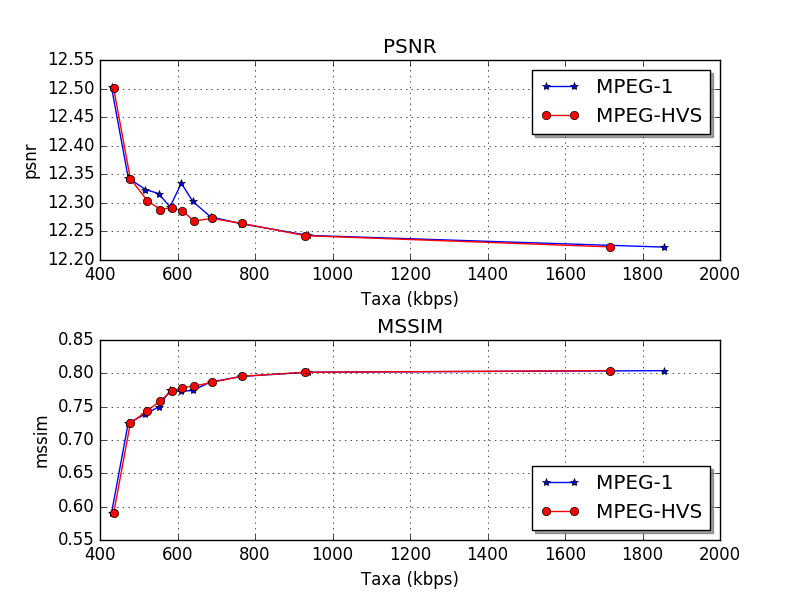
\includegraphics[width=.5\textwidth]{./Figures/png/akiyo_cif_vs_hvs.png}}
\subfigure[Ice.]{\label{fig:mssim_ice}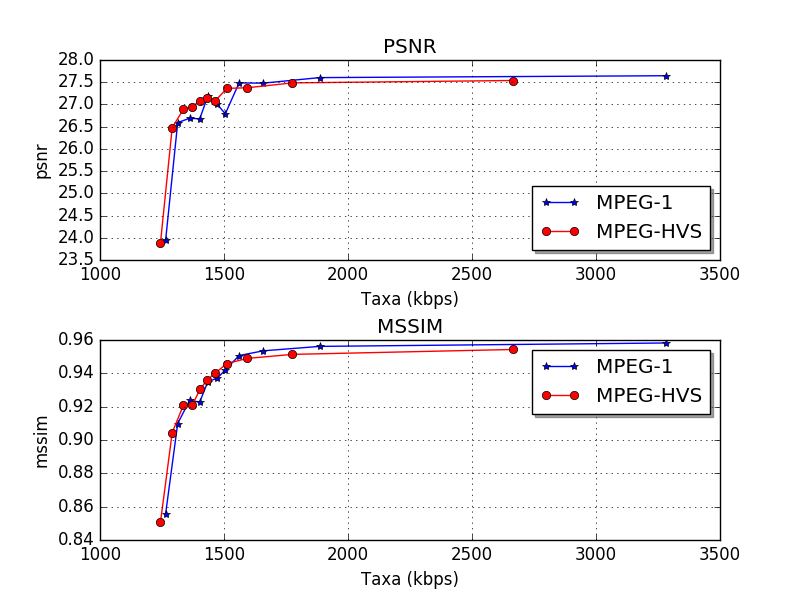
\includegraphics[width=.5\textwidth]{./Figures/png/ice_cif_vs_hvs.png}}
\subfigure[Stefan.]{\label{fig:mssim_stefan}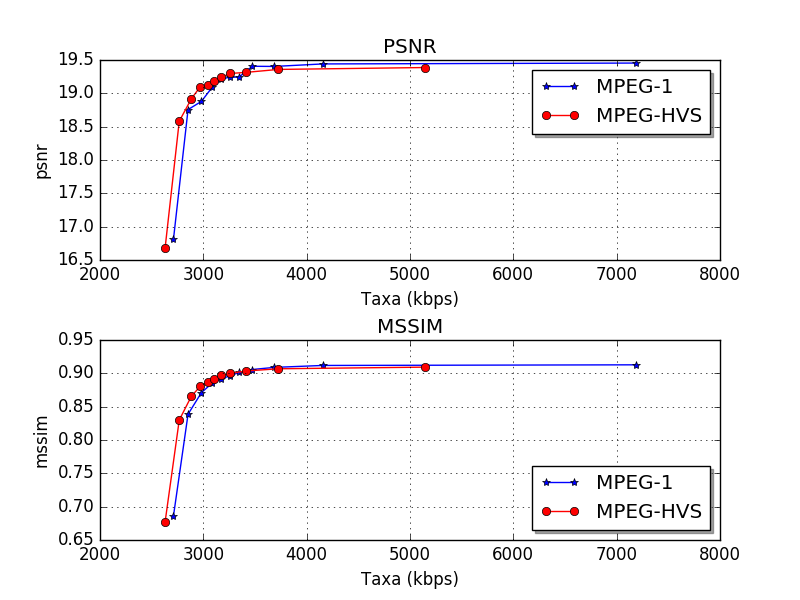
\includegraphics[width=.5\textwidth]{./Figures/png/stefan_cif_vs_hvs.png}}
\subfigure[Foreman.]{\label{fig:mssim_foreman}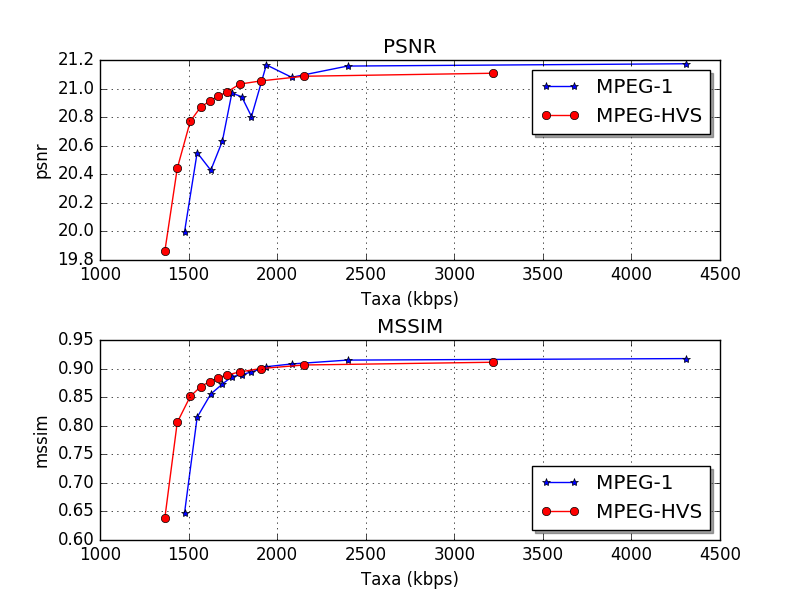
\includegraphics[width=.5\textwidth]{./Figures/png/foreman_cif_vs_hvs.png}}
\caption{Comparativo dos valores de MSSIM e PSNR pelos codecs padrão e perceptual.}
\end{figure}

\begin{figure}[!ht]\label{MSSIM}
\subfigure[]{\label{visu_standard}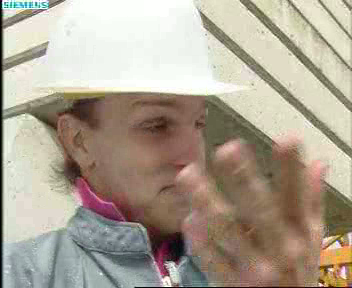
\includegraphics[width=.5\textwidth, height=.4\textwidth]{./Figures/png/foreman_155_1500.png}}
\subfigure[]{\label{visu_standard_cut}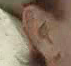
\includegraphics[width=.5\textwidth, height=.4\textwidth]{./Figures/png/foreman_155_1500_cut.png}}
\subfigure[]{\label{visu_perceptual}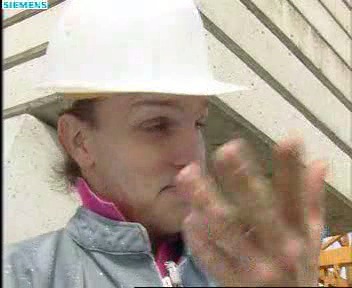
\includegraphics[width=.5\textwidth, height=.4\textwidth]{./Figures/png/foreman_hvs_155_1500.png}}
\subfigure[]{\label{visu_perceptual_cut}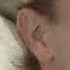
\includegraphics[width=.5\textwidth, height=.4\textwidth]{./Figures/png/foreman_hvs_155_1500_cut.png}}
\caption{Comparativo entre os codecs padrão, (a) e (b), e perceptual, (c) e (d).}
\label{comp_visual}
\end{figure}

\newpage

Utilizando a tabela ponderada (Fig. \ref{MSSIM_fase2}) de quantização na codificação das imagens P e B, os resultados obtidos são ainda mais interessantes. Diferentemente do que foi apontado em \cite{ghanbari2003standard}, pois essa adaptação gerou taxas (kbps) muito menores em comparação aos codificadores padrão e perceptual.

\begin{figure}[!ht]\label{MSSIM_fase2}
\subfigure[Akiyo.]{\label{fig:mssim_akiyo2}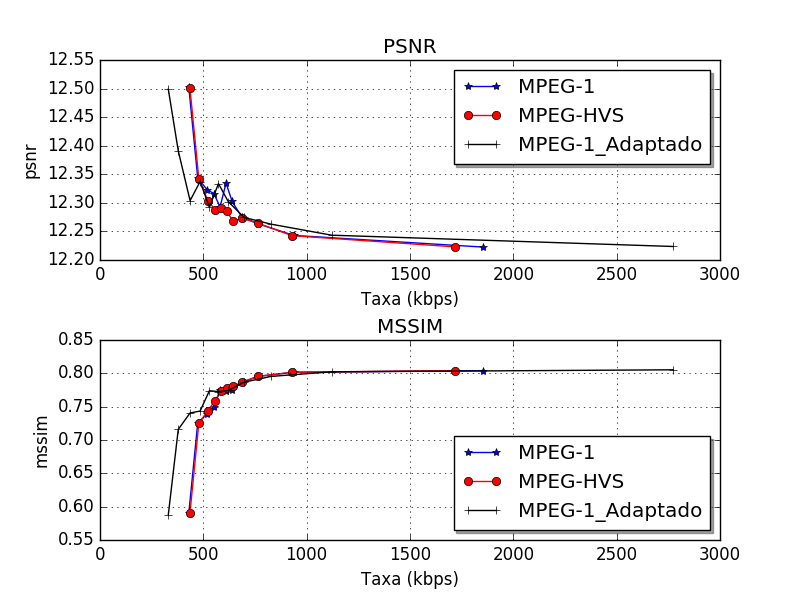
\includegraphics[width=.5\textwidth]{./Figures/png/akiyo_fase2.png}}
\subfigure[Ice.]{\label{fig:mssim_ice2}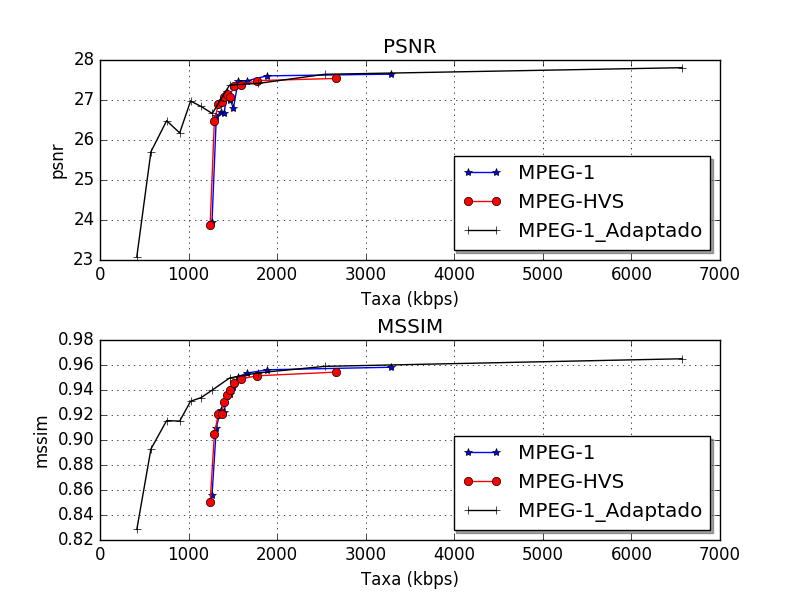
\includegraphics[width=.5\textwidth]{./Figures/png/ice_fase2.png}}
\subfigure[Stefan.]{\label{fig:mssim_stefan2}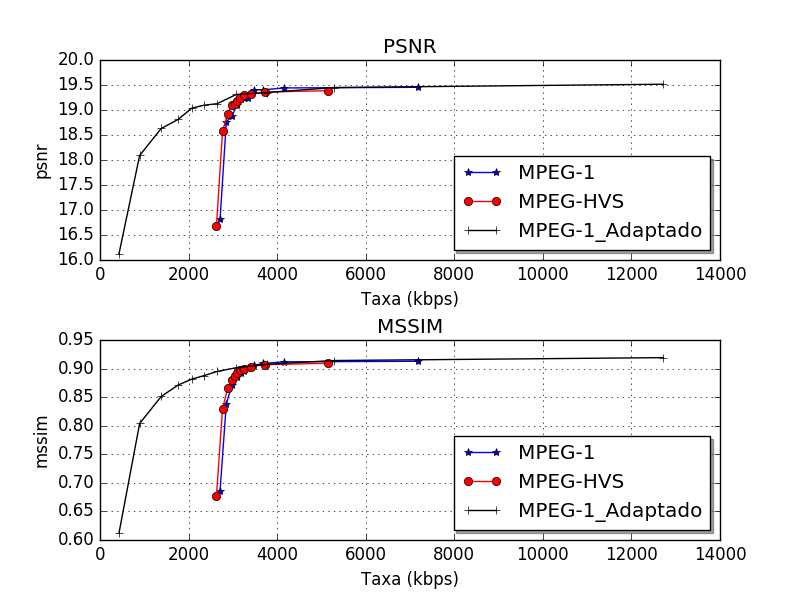
\includegraphics[width=.5\textwidth]{./Figures/png/stefan_fase2.png}}
\subfigure[Foreman.]{\label{fig:mssim_foreman2}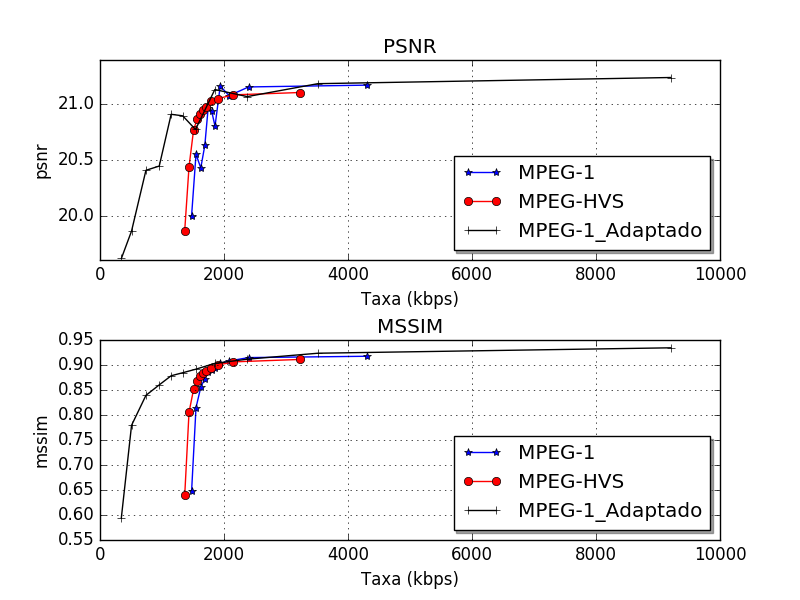
\includegraphics[width=.5\textwidth]{./Figures/png/foreman_fase2.png}}
\caption{Comparativo dos valores de MSSIM e PSNR pelos codecs padrão, padrão adaptado e perceptual.}
\end{figure}

Apesar dos resultados gerados pela utilização da tabela de quantização ponderada, em dentrimento da plana, terem se destacado como os mais eficienties, ainda não há, nesse trabalho, uma explicação plausível para esse comportamento.